\documentclass{beamer}
\usepackage{xcolor}
\usepackage{amsmath}
\usepackage{amsfonts}
\usepackage{amssymb}
\usepackage{graphicx}
\graphicspath{ {images/} }
\usetheme[titlepagelogo=logo-ctut,
  				color=blue,
		  		language=vietnamese,
		  		coding=utf8,
  				bullet=circle,
  				secondsupervisor=false,
  				assistantsupervisor=false,
  				secondassistantsupervisor=false,
  				secondcandidate=true,
  				notshowauthor = true,
  				]{TorinoTh}
\author[SƠ ĐỒ NỐI ĐIỆN]{Nguyễn Văn Đình -- Thi Minh Nhựt}
\rel{ThS. Quách Hữu Lượng}
\title{\textbf{CHỦ ĐỀ BÁO CÁO HỆ THỐNG ĐIỆN\hspace{.1cm}\\SƠ ĐỒ NỐI ĐIỆN}}
\ateneo{{\small \textbf{TRƯỜNG ĐẠI HỌC KỸ THUẬT -- CÔNG NGHỆ CẦN THƠ}}}
\date{\today}
\secondcandidate{Phạm Thanh Quý -- Liên Thái Trường\\ \vspace{.5em}  -- Lư Anh Tuấn}
\setrellabel{Giảng viên hướng dẫn}
\setcandidatelabel{Nhóm sinh viên thực hiện}
\begin{document}
\titlepageframe

\begin{tframe}{\textbf{Nội dung trình bày}}
\tableofcontents
\end{tframe}
\section{Các khái niệm mở đầu}
\begin{frame}{\textbf{Khái niệm và yêu cầu về sơ đồ nối điện}}
\begin{block}{\textbf{Khái niệm}}
\emph{Sơ đồ nối điện} là tập hợp: máy phát, máy biến áp, đường dây, thanh cái, các thiết bị thao tác: máy cắt, dao cách ly,\ldots
\end{block}

\begin{block}{\textbf{Yêu cầu}}
\begin{itemize}
\item Vị trí, vai trò của nhà máy điện và trạm biến áp.
\item Độ tin cậy cung cấp điện.
\item Sơ đồ đơn giản, linh hoạt, thuận tiện thao tác, an toàn phục vụ.
\item Tính kinh tế.
\end{itemize}
\end{block}
\end{frame}

\section{Sơ đồ nối điện}
\subsection{Các dạng sơ đồ nối điện cơ bản}
\begin{tframe}{\textbf{Các dạng sơ đồ nối điện cơ bản}}
Người ta phân loại dựa vào \highlight{số lượng thanh góp}, \highlight{số lượng máy cắt} có trong sơ đồ. Chia làm các nhóm sau:
\begin{itemize}
\item \textbf{\emph{Nhóm 1}}: mỗi phần tử \alert{chỉ đi qua một máy cắt}, máy cắt đóng thì làm việc, cắt thì phần tử ngưng làm việc. Phụ thộc vào \emph{số lượng thanh góp}.
\item \textbf{\emph{Nhóm 2}}: mỗi phần tử được cung cấp hai phía \alert{qua qua máy cắt}, \emph{một máy cắt hỏng} thì \emph{không làm mất điện}. Sơ đồ thuộc nhóm này \emph{đáp ứng được yêu cầu cao hơn}.
\item \textbf{\emph{Nhóm 3}}: \alert{một hoặc hai mạch} trên sơ đồ \alert{không đặt máy cắt} mà \alert{chỉ đặt dao cách ly}. Sơ đồ nhóm này \emph{đáp ứng yêu cầu thấp}.
\end{itemize}
\end{tframe}
\subsection{Sơ đồ hệ thống thanh góp}
\begin{frame}{\textbf{Hệ thống một thanh góp không phân đoạn}}
\begin{columns}
\column{0.5\textwidth}
\begin{figure}[h]
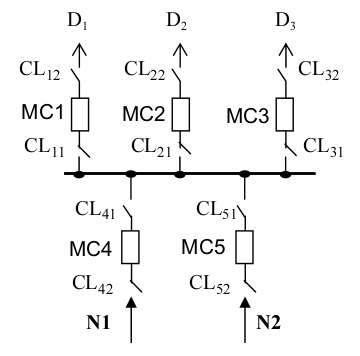
\includegraphics[width=5cm, height=5cm]{mtgkpd}
\caption{Sơ đồ hệ thống một thanh góp không phân đoạn}
\end{figure}

\column{0.5\textwidth}
\begin{itemize}
\item<1-> \textbf{Mô tả sơ đồ}
\item<2-> \textbf{Thao tác sửa chữa}
\begin{itemize}
\item<3-> \emph{Kiểm tra đường dây $D2$}: \uncover<4->{cắt máy cắt $MC2\rightarrow$ cắt dao cách ly $CL_{22}\rightarrow$ thực hiện thao tác sửa chữa đường dây an toàn.}
\item<3-> \emph{Ngắn mạch đường dây $D2$}: \uncover<5->{relay bảo vệ đưa tín $\rightarrow$ cắt máy cắt $MC2\rightarrow$ cắt dao cách ly $CL_{22}\rightarrow$ thực hiện thao tác sửa chữa đường dây an toàn.}
\end{itemize}
\end{itemize}
\end{columns}
\end{frame}


\begin{frame}{\textbf{Hệ thống một thanh góp không phân đoạn (tt)}}
\begin{columns}
\column{0.5\textwidth}
\begin{figure}[h]
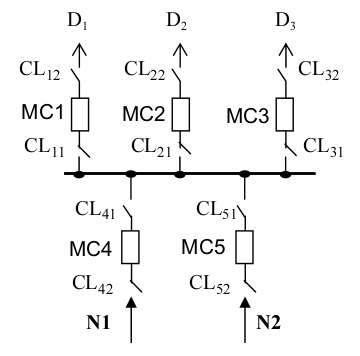
\includegraphics[width=5cm, height=5cm]{mtgkpd}
\caption{Sơ đồ hệ thống một thanh góp không phân đoạn}
\end{figure}

\column{0.5\textwidth}
\begin{itemize}
\item \textbf{Mô tả sơ đồ}
\item \textbf{Thao tác sửa chữa}
\begin{itemize}
\item <1-> \emph{Sửa chữa thanh góp}: \uncover<2->{cắt máy cắt (theo thứ tự kém quan trọng), ví dụ: $MC1,MC2$, $MC3\rightarrow$ cắt tất cả các máy cắt nối vào nguồn $MC4,MC5\rightarrow$ cắt dao cách ly nối vào thanh góp: $CL_{11},CL_{21},CL_{31}, CL_{41}$, $CL_{51}\rightarrow$ thực hiện thao tác sửa chữa thanh góp: nối đất an toàn,\ldots}
\end{itemize}
\end{itemize}
\end{columns}
\end{frame}

\begin{frame}{\textbf{Hệ thống một thanh góp không phân đoạn (tt)}}
\begin{columns}
\column{0.5\textwidth}
\begin{figure}[h]
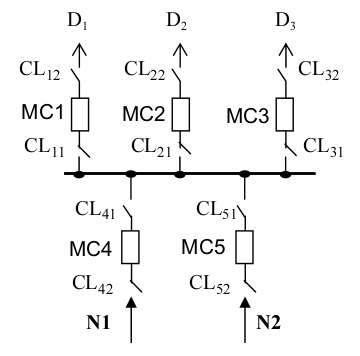
\includegraphics[width=5cm, height=5cm]{mtgkpd}
\caption{Sơ đồ hệ thống một thanh góp không phân đoạn}
\end{figure}

\column{0.5\textwidth}
\begin{itemize}
\item \textbf{Mô tả sơ đồ}
\item  \textbf{Thao tác sửa chữa}
\begin{itemize}
\item<1-> \emph{Ngắn mạch thanh góp}: \uncover<2->{relay bảo vệ đưa tín hiệu $\rightarrow$ máy cắt nguồn $MC4,MC5$ và máy cắt đường  dây $MC2,MC3\rightarrow$ cắt máy cắt mà relay bảo vệ chưa cắt $MC1\rightarrow$ cắt dao cách ly thanh góp $CL_{11}$, $CL_{21}$, $CL_{31}$, $CL_{41}$, $CL_{51}\rightarrow$ thực hiện thao tác sửa chữa thanh góp an toàn.}
\end{itemize}
\end{itemize}
\end{columns}
\end{frame}

\begin{frame}{\textbf{Hệ thống một thanh góp không phân đoạn (tt)}}
\begin{columns}
\column{0.5\textwidth}
\begin{figure}[h]
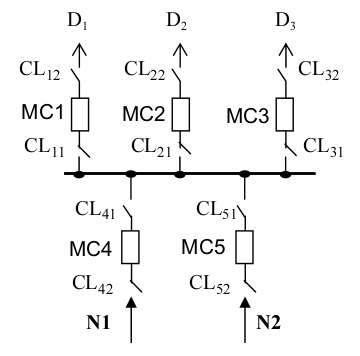
\includegraphics[width=5cm, height=5cm]{mtgkpd}
\caption{Sơ đồ hệ thống một thanh góp không phân đoạn}
\end{figure}

\column{0.5\textwidth}
\begin{itemize}
\item \textbf{Mô tả sơ đồ}
\item  \textbf{Thao tác sửa chữa}
\item \textbf{Khôi phục lại sơ đồ làm việc}
\begin{itemize}
\item<1-> Khi có sự cố trên thanh góp thì toàn bộ sơ đồ mất điện.
\item<2-> \emph{Khôi phục lại sơ đồ}: \uncover<3->{mở nối đất an toàn $\rightarrow$ đóng các dao cách ly thanh góp $\rightarrow$ đóng máy cắt nguồn nối vào thanh góp $\rightarrow$ đóng các máy cắt đường dây theo thứ tự quan trọng trước.}
\item<4-> Dao cách ly phải đặt đúng chiều.
\end{itemize}
\end{itemize}
\end{columns}
\end{frame}


\begin{frame}{\textbf{Hệ thống một thanh góp có một phân đoạn}}
\begin{columns}
\column{0.4\textwidth}
\begin{figure}[h]
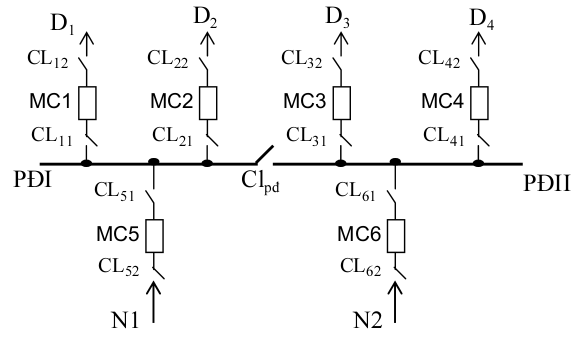
\includegraphics[width=4cm, height=5cm]{mtgcpd}
\caption{Sơ đồ hệ thống một thanh góp có phân đoạn}
\end{figure}

\column{0.6\textwidth}
\begin{itemize}
\item \textbf{Mô tả sơ đồ}
\item  \textbf{Thao tác sửa chữa}
\begin{itemize}
\item<1-> \emph{Phân đoạn $I$ -- giả sử dao cách ly đóng}: \uncover<2->{cắt máy cắt mạch đường dây và máy cắt mạch nguồn nối vào phân đoạn $I$ $\rightarrow$ cắt dao cách ly thanh góp nối vào phân đoạn $I$ $\rightarrow$ cắt dao cách ly phân đoạn $\rightarrow$ thực hiện sửa chữa phân đoạn $I$ an toàn.}
\end{itemize}
\end{itemize}
\end{columns}
\end{frame}

\begin{frame}{\textbf{Hệ thống một thanh góp có một phân đoạn (tt)}}
\begin{columns}
\column{0.4\textwidth}
\begin{figure}[h]
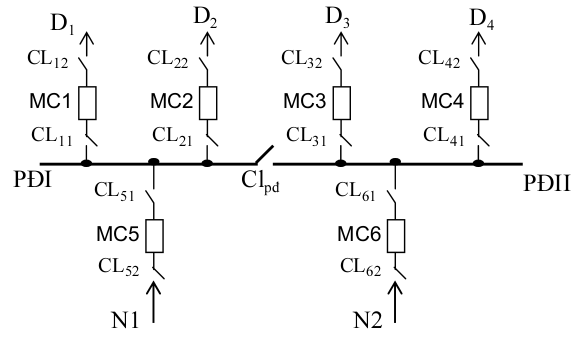
\includegraphics[width=4cm, height=5cm]{mtgcpd}
\caption{Sơ đồ hệ thống một thanh góp có phân đoạn}
\end{figure}

\column{0.6\textwidth}
\begin{itemize}
\item \textbf{Mô tả sơ đồ}
\item  \textbf{Thao tác sửa chữa}
\begin{itemize}
\item<1-> \emph{Ngắn mạch thanh góp phân đoạn $I$ -- giả sử dao cách ly đóng}: \uncover<2->{relay bảo vệ đưa tín hiệu cắt máy cắt nguồn $\rightarrow$ cắt các máy cắt mà relay bảo vệ chưa cắt $\rightarrow$ cắt tất cả các dao cách ly thanh góp $\rightarrow$ mở dao cách ly phân đoạn $\rightarrow$ chỉnh định thời gian của relay bảo vệ cắt máy cắt nguồn về giá trị nhỏ nhất $\rightarrow$ đóng máy cắt $MC1$ kiểm tra có phải ngắn mạch trên phân đoạn $I$ không? Giả sử biết, sửa chữa xong ngắn mạch phân đoạn $I$.}
\end{itemize}
\end{itemize}
\end{columns}
\end{frame}

\begin{frame}{\textbf{Hệ thống một thanh góp có một phân đoạn (tt)}}
\begin{columns}
\column{0.4\textwidth}
\begin{figure}[h]
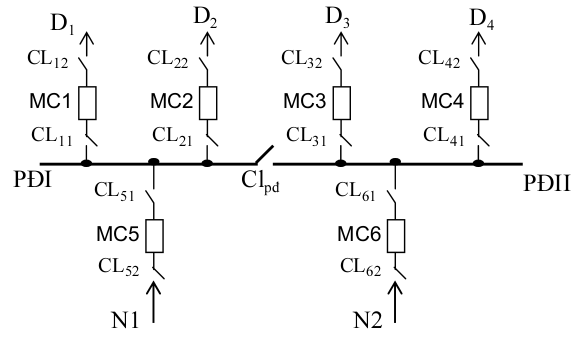
\includegraphics[width=4cm, height=5cm]{mtgcpd}
\caption{Sơ đồ hệ thống một thanh góp có phân đoạn}
\end{figure}

\column{0.6\textwidth}
\begin{itemize}
\item \textbf{Mô tả sơ đồ}
\item  \textbf{Thao tác sửa chữa}
\item  \textbf{Thao tác khôi phục}
\begin{itemize}
\item<1-> \emph{Khôi phục hoạt động bình thường của phân đoạn $II$}: \uncover<2->{đóng máy cắt nguồn của phân đoạn $II$ $\rightarrow$ chỉ định thời gian của relay bảo vệ như làm việc bình thường $\rightarrow$ đóng máy cắt mạch đường dây theo thứ tự ưu tiên.}
\item<1-> \emph{Khôi phục hoạt động của phân đoạn $I$ đã sửa xong}: \uncover<3->{cắt tất cả máy cắt nối vào phân đoạn $II$ $\rightarrow$ đóng dao cách ly phân đoạn.}
\end{itemize}
\end{itemize}
\end{columns}
\end{frame}

\begin{frame}{\textbf{Hệ thống một thanh góp có hai phân đoạn }}
\begin{columns}
\column{0.4\textwidth}
\begin{figure}[h]
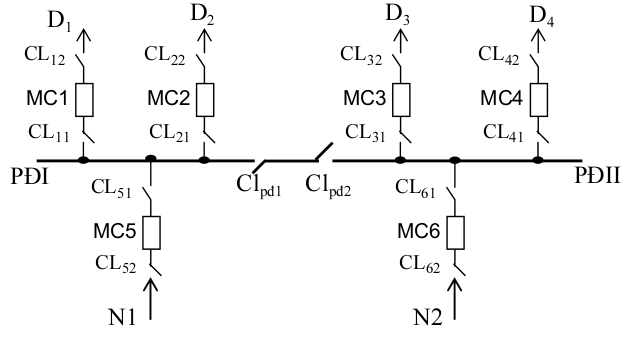
\includegraphics[width=4cm, height=5cm]{mtgc2pd}
\caption{Sơ đồ hệ thống một thanh góp có hai phân đoạn}
\end{figure}

\column{0.6\textwidth}
\begin{itemize}
\item Ở sơ đồ trước, khi sửa chữa dao cách ly phân đoạn thì cả hai phân đoạn đều mất điện. Sơ đồ hình bên, cho phép sửa chữa từng dao cách ly mà chỉ có một phân đoạn mất điện.
\item  \textbf{Thao tác sửa chữa}
\begin{itemize}
\item<1-> \emph{Sửa chửa dao cách ly phân đoạn $I$}: \uncover<2->{cắt tất cả máy cắt nối vào phân đoạn $I$ $\rightarrow$ cắt tất cả dao cách ly thanh góp nối vào phân đoạn $I$ $\rightarrow$ cắt dao cách ly $CL_{pd1}$ $\rightarrow$ thực hiện biện pháp sửa chữa an toàn.}
\end{itemize}
\end{itemize}
\end{columns}
\end{frame}

\begin{frame}{\textbf{Hệ thống một thanh góp có hai phân đoạn bằng máy cắt}}
\begin{columns}
\column{0.5\textwidth}
\begin{figure}[h]
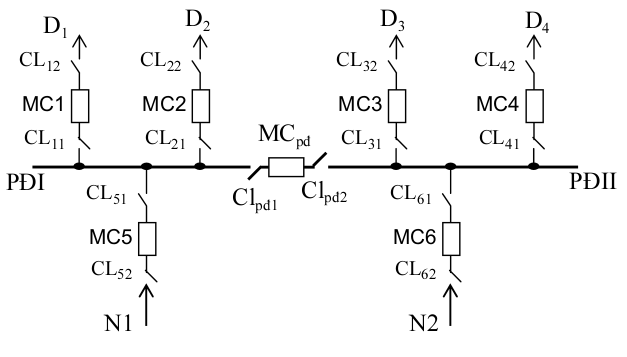
\includegraphics[width=4cm, height=4cm]{pdbmc}
\caption{Sơ đồ hệ thống một thanh góp có hai phân đoạn bằng máy cắt}
\end{figure}

\column{0.5\textwidth}
\begin{itemize}
\item \textbf{Mô tả}
\item  \textbf{Thao tác sửa chữa}
\begin{itemize}
\item<1-> \emph{Sửa chữa ngắn mạch phân đoạn $I$}: \uncover<2->{cắt tất cả máy cắt nguồn nối vào phân đoạn $I$  \quad $\rightarrow$ phân đoạn $I$ mất nguồn, phân đoạn $II$ còn nguồn $\rightarrow$ sửa xong phân đoạn $I$ $\rightarrow$ đóng $CL_{pd1}$, $CL_{pd2}$, $MC_{pd}$ $\rightarrow$ đóng dao cách ly 2 đầu máy cắt $MC5$ $\rightarrow$ đóng máy cắt $MC5$ $\rightarrow$ nối đường dây theo thứ tự ưu tiên vào trước.}
\end{itemize}
\end{itemize}
\end{columns}
\end{frame}

\subsection{Sơ đồ cung cấp điện dự phòng cho phụ tải quan trọng}
\begin{frame}{\textbf{Sơ đồ cung cấp điện cho phụ tải quan trọng}}
\begin{columns}
\column{0.5\textwidth}
\begin{figure}[h]
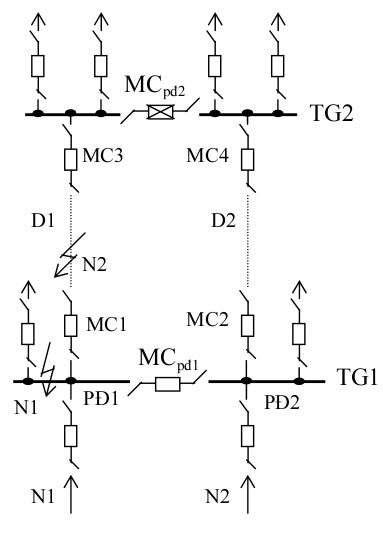
\includegraphics[width=4cm, height=5cm]{ccddp}
\caption{Sơ đồ cung cấp điện dự phòng cho phụ tải quan trọng}
\end{figure}

\column{0.5\textwidth}
\begin{itemize}
\item \textbf{Mô tả}
\item  \textbf{Thao tác sửa chữa}
\begin{itemize}
\item<1-> \emph{Khi $N2$ ngắn mạch}: \uncover<2->{Máy cắt $MC1$, $MC3$ cắt $\rightarrow$ phân đoạn $I$ của $TG2$ mất điện $\rightarrow$ máy cắt $MC_{pd2}$ đóng (tác động của nguồn dự trữ) $\rightarrow$ phân đoạn $I$ được cung cấp điện từ đường dây $D2$.}
\item<1-> \emph{Khi ngắn mạch $N1$}: \uncover<3->{cắt máy cắt $MC_{pd1}$ và các máy cắt liên quan $TG1$ $\rightarrow$ máy cắt $MC_{pd2}$ tự đóng lại}
\end{itemize}
\end{itemize}
\end{columns}
\end{frame}

\subsection{Sơ đồ bộ máy biến áp -- đường dây}

\begin{frame}{\textbf{Sơ đồ bộ máy biến áp -- đường dây}}
\begin{columns}
\column{0.5\textwidth}
\begin{figure}[h]
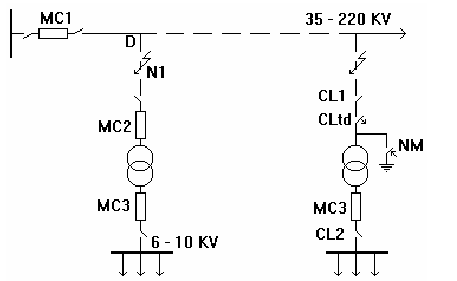
\includegraphics[width=4cm, height=4cm]{sdbmba}
\caption{Sơ đồ của các trạm biến áp nối vào đường dây}
\end{figure}

\column{0.5\textwidth}
\begin{itemize}
\item \textbf{Mô tả}
\item  \textbf{Thao tác sửa chữa}
\begin{itemize}
\item<1-> \emph{Ngắn mạch tại $N1$}: $MC1$ và $MC2$ cắt.
\item<1-> \emph{Sự cố máy biến áp}: $MC2$ và $MC3$ cắt.
\item<1-> \emph{Ngắn mạch máy biến áp}: \uncover<2->{relay bảo vệ cắt máy cắt $MC_3$ $\rightarrow$ đưa tín hiệu cắt máy cắt $MC1$ $\rightarrow$ dao cắt $CL_{td}$ mở ra $\rightarrow$ tác động của thiết bị tự đóng lại $\rightarrow$ đóng $MC1$.}
\item<1-> \emph{Đóng máy biến áp}: \uncover<3->{đóng $CL1$ và $CL2$ $\rightarrow$ đóng $CL_{td}$ $\rightarrow$ đóng cắt $MC3.$}  
\end{itemize}
\end{itemize}
\end{columns}
\end{frame}

\subsection{Sơ đồ cầu}
\begin{frame}{\textbf{Sơ đồ cầu ngoài}}
\begin{columns}
\column{0.5\textwidth}
\begin{figure}[h]
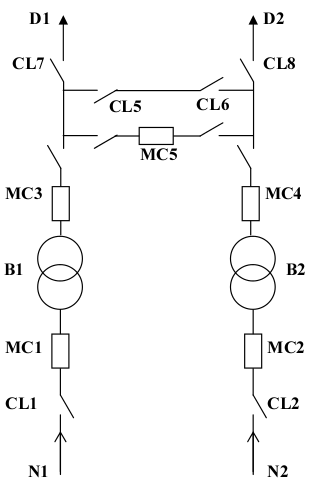
\includegraphics[width=4cm, height=5cm]{sdcn}
\caption{Sơ đồ cầu ngoài}
\end{figure}

\column{0.5\textwidth}
\begin{itemize}
\item \textbf{Mô tả}
\item  \textbf{Thao tác sửa chữa}
\begin{itemize}
\item<1-> \emph{Sửa máy cắt $MC5$}: \uncover<2->{đóng $CL5$, $CL6$ $\rightarrow$ cắt $MC5$ $\rightarrow$ cắt $CL5$, $CL6$ $\rightarrow$ thực hiện thao tác sửa chữa an toàn.}
\item<1-> \emph{Sửa máy biến áp $B1$}: \uncover<3->{cắt $MC1$, $MC3$ $\rightarrow$ mở 2 dao cách ly 2 đầu máy cắt $\rightarrow$ thực hiện thao tác sửa chữa an toàn.}
\end{itemize}
\end{itemize}
\end{columns}
\end{frame}

\begin{frame}{\textbf{Sơ đồ cầu ngoài (tt)}}
\begin{columns}
\column{0.5\textwidth}
\begin{figure}[h]
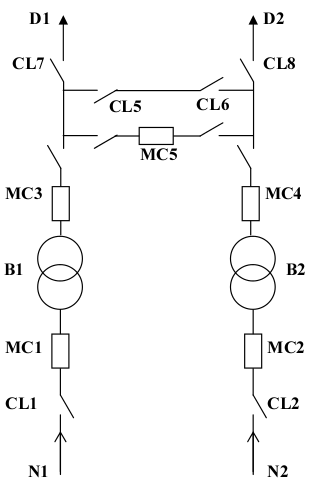
\includegraphics[width=4cm, height=5cm]{sdcn}
\caption{Sơ đồ cầu ngoài}
\end{figure}

\column{0.5\textwidth}
\begin{itemize}
\item \textbf{Mô tả}
\item  \textbf{Thao tác sửa chữa}
\begin{itemize}
\item<1-> \emph{Sửa máy đường dây $D1$}: \uncover<2->{cắt $MC3$, $MC5$ $\rightarrow$ cắt $CL7$ $\rightarrow$ đóng $MC3$, $MC5$ $\rightarrow$ thực hiện thao tác sửa chữa an toàn.}
\item<1-> \emph{Đóng lại đường dây $D1$}: \uncover<3->{tháo nối đất an toàn $\rightarrow$ cắt $MC3$, $MC5$ $\rightarrow$ đóng $CL7$ $\rightarrow$ đóng $MC3$, $MC5$}
\end{itemize}
\end{itemize}
\end{columns}
\end{frame}

\begin{frame}{\textbf{Sơ đồ cầu trong}}
\begin{columns}
\column{0.5\textwidth}
\begin{figure}[h]
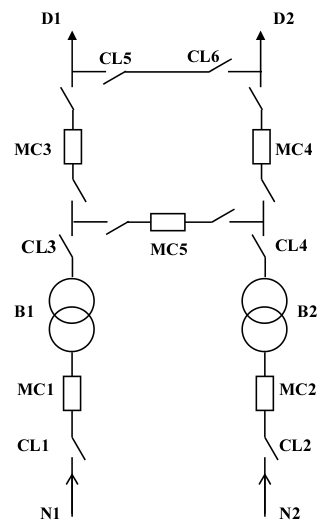
\includegraphics[width=4cm, height=4cm]{sdct}
\caption{Sơ đồ cầu trong}
\end{figure}

\column{0.5\textwidth}
\begin{itemize}
\item \textbf{Mô tả}
\item  \textbf{Thao tác sửa chữa}
\begin{itemize}
\item<1-> \emph{Sửa máy đường dây $D1$}: \uncover<2->{cắt $MC3$ $\rightarrow$ cắt dao cách ly hai đầu $MC3$ $\rightarrow$ thực hiện thao tác sửa chữa an toàn.}
\item<1-> \emph{Sự cố máy biến áp $B1$}: \uncover<3->{cắt $MC1$, $MC3$, $MC5$ $\rightarrow$ $D1$ mất điện, để đóng lại $\rightarrow$ cắt $CL1$ $\rightarrow$ đóng $MC3$, $MC5$ $\rightarrow$ thực hiện thao tác sửa chữa an toàn.}
\end{itemize}
\end{itemize}
\end{columns}
\end{frame}

\begin{frame}{\textbf{Sơ đồ cầu trong  (tt)}}
\begin{columns}
\column{0.5\textwidth}
\begin{figure}[h]
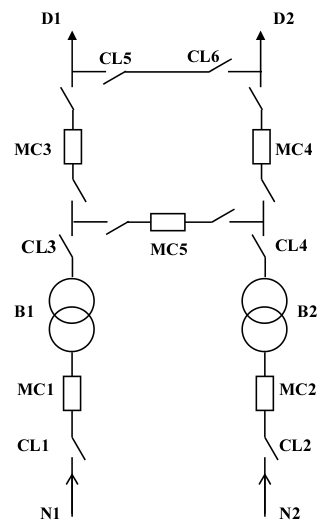
\includegraphics[width=4cm, height=4cm]{sdct}
\caption{Sơ đồ cầu trong}
\end{figure}

\column{0.5\textwidth}
\begin{itemize}
\item \textbf{Mô tả}
\item  \textbf{Thao tác sửa chữa}
\begin{itemize}
\item<1-> \emph{Sửa máy cắt $MC3$}: \uncover<2->{đóng dao cách ly đang mở $\rightarrow$ cắt $MC3$ $\rightarrow$ cắt dao cách ly 2 đầu $MC3$ $\rightarrow$ thực hiện thao tác sửa chữa an toàn.}
\item<1-> \emph{Sửa máy cắt $MC5$}: \uncover<3->{đóng $CL5$, $CL6$ $\rightarrow$ cắt $MC5$ $\rightarrow$ cắt dao cách ly 2 đầu $MC5$ $\rightarrow$ thực hiện thao tác sửa chữa an toàn.}
\end{itemize}
\end{itemize}
\end{columns}
\end{frame}

\subsection{Sơ đồ đa giác}

\begin{frame}{\textbf{Sơ đồ tam giác}}
\begin{columns}
\column{0.5\textwidth}
\begin{figure}[h]
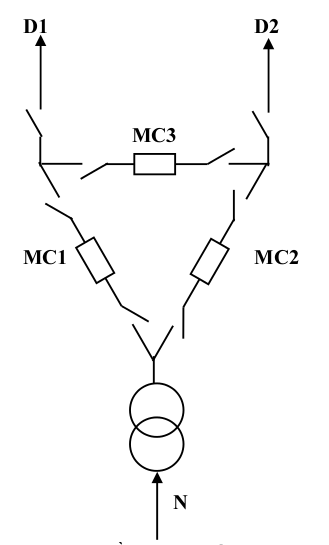
\includegraphics[width=4cm, height=5cm]{tamgiac}
\caption{Sơ đồ tam giác}
\end{figure}

\column{0.5\textwidth}
\begin{itemize}
\item \textbf{Mô tả}
\item  \textbf{Thao tác sửa chữa}
\begin{itemize}
\item<1-> \emph{Kiểm tra máy cắt $MC1$}: \uncover<2->{cắt máy cắt $MC1$ $\rightarrow$ mở hai đầu máy cắt $\rightarrow$ thực hiện kiểm tra máy cắt an toàn $\rightarrow$ đường dây $D1$ vẫn được bảo vệ bởi máy cắt $MC3$.}
\item<1-> \emph{Đường dây $D1$}: \uncover<3->{máy cắt $MC1$, $MC3$ cắt $\rightarrow$ mở dao cách ly trên $D1$ $\rightarrow$ duy trì máy cắt dự trữ đóng $MC1$ và $MC3$.}
\end{itemize}
\end{itemize}
\end{columns}
\end{frame}

\begin{frame}{\textbf{Sơ đồ tứ giác}}
\begin{columns}
\column{0.5\textwidth}
\begin{figure}[h]
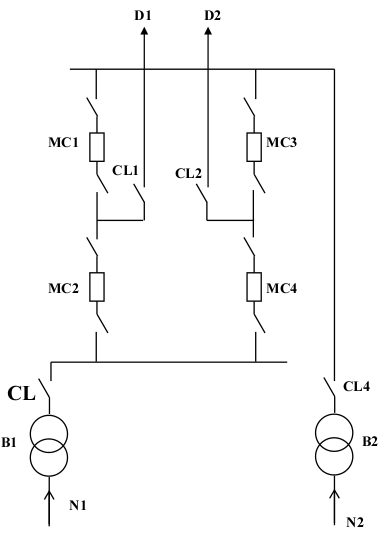
\includegraphics[width=4cm, height=5cm]{tugiac}
\caption{Sơ đồ tứ giác}
\end{figure}

\column{0.5\textwidth}
\begin{itemize}
\item \textbf{Mô tả}
\item  \textbf{Thao tác sửa chữa}
\begin{itemize}
\item<1-> \emph{Kiểm tra máy cắt $MC1$}: \uncover<2->{cắt máy cắt $MC1$, $MC2$ $\rightarrow$ mở hai đầu máy cắt $\rightarrow$ thực hiện kiểm tra máy cắt an toàn.}
\item<1-> \emph{Đường dây $D1$}: \uncover<3->{máy cắt $MC1$, $MC2$ cắt $\rightarrow$ mở dao cách ly $CL1$ $\rightarrow$ đóng $MC1$ và $MC2$ để duy trì mạch vòng kín.}
\item<1-> \emph{Ngắn mạch trên $D1$}: \uncover<4->{nếu $MC1$ hoặc $MC2$ không cắt $\rightarrow$ $MC3$ cắt $\rightarrow$  máy biến áp $B1$ ngừng làm việc.}
\end{itemize}
\end{itemize}
\end{columns}
\end{frame}
\section{Tài liệu tham khảo}
\begin{frame}{\textbf{Tài liệu tham khảo}}
\begin{itemize}
\item \textbf{Bài  giảng Hệ thống điện} -- Thầy Quách Hữu Lượng -- Đại học Kỹ thuật -- Công nghệ Cần Thơ.
\item \textbf{Giáo trình Phần điện trong Nhà máy điện và Trạm biến áp} -- Nhóm Nhà máy điện -- Bộ môn Hệ thống điện -- ĐHBK Đà Nẵng.
\item \textbf{Soure code \LaTeX{} Thesis theme for Beamer} -- Beamer2Thesis -- \textsf{http://cfiandra.github.io/Beamer2Thesis/}
\end{itemize}
\end{frame}
\end{document}
